\documentclass[10pt, a4paper]{article}

\usepackage{ctex}
\usepackage{xeCJK}
\usepackage{caption}
\usepackage{geometry}
\geometry{
    left = 0.6in,
    right = 0.6in,
    top = 0.8in,
    bottom = 1.0in
}
\usepackage{amssymb}
\usepackage{amsbsy}
\usepackage{amsmath}
\usepackage{xcolor}
\usepackage{mathrsfs}
\usepackage{graphicx}
\usepackage{tasks}
\settasks{
    label = \Alph*. ,
    label-width = 16pt
}

\newcommand{\Title}[3]{
    \begin{center}
        \Large \textbf{中国电子学会 #1~年~#2~月 Scratch~#3级考试}
    \end{center}
}
\newcommand{\TimeAndName}[1]{
    \begin{center}
        考试时间:~#1~ 分钟 \qquad\qquad\qquad\qquad 姓名:\underline{\quad\quad\quad\quad}
    \end{center}
}
\begin{document}
    \Title{2021}{12}{一}
    
    \TimeAndName{60}
    
    \vspace{1cm}
    {\noindent\heiti 第一部分、单选题(共 25 题,每题 2 分,共50分.)}

    \begin{enumerate}
        % 1
        \item 点击下列哪个按钮,可以让正在运行的程序停下来?(\qquad)
        \begin{tasks}(4)
            \task 
\includegraphics[width=.05\textwidth]{1a.jpg}
            \task 
\includegraphics[width=.05\textwidth]{1b.jpg}
            \task 
\includegraphics[width=.05\textwidth]{1c.jpg}
            \task 
\includegraphics[width=.05\textwidth]{1d.jpg}
        \end{tasks}

        % 2
        \item 如下图,小乔完成了一个编程作品后,点击“文件”中的“保存到电脑”将作品保存到本地,不修改文件名字,直接点击保存。以下哪个选项是作品文件的名字?(\qquad)
        \begin{tasks}(2)
            \task 旋转的星星.sb3
            \task 旋转的星星.sprite3
            \task 一闪一闪亮晶晶.sb3
            \task 一闪一闪亮晶晶.sprite3
        \end{tasks}

        % 3
        \item 点击下列哪个按钮可以绘制一个角色?(\qquad)
        \begin{tasks}(4)
            \task 
\includegraphics[width=.05\textwidth]{3a.jpg}
            \task 
\includegraphics[width=.05\textwidth]{3b.jpg}
            \task 
\includegraphics[width=.05\textwidth]{3c.jpg}
            \task 
\includegraphics[width=.05\textwidth]{3d.jpg}
        \end{tasks}

        \begin{figure}[htbp]
            \centering
            \begin{minipage}[t]{.35\textwidth}
                \centering
                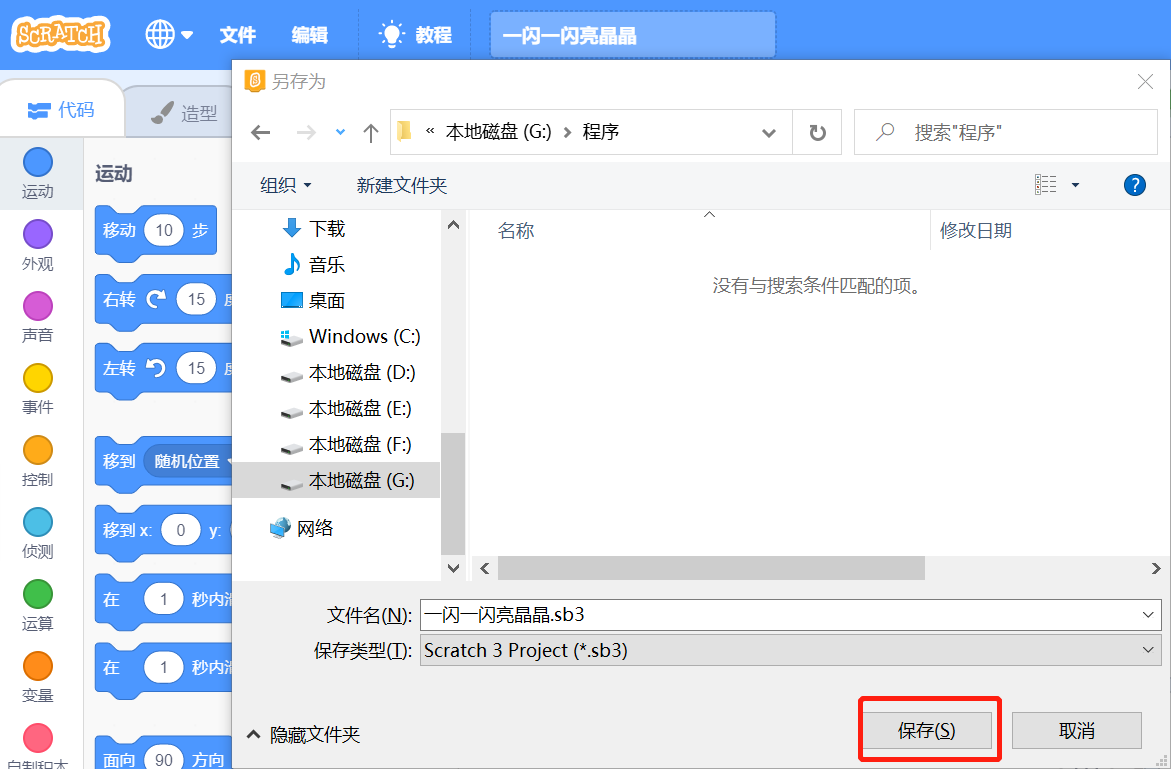
\includegraphics[width=1\textwidth]{2.png}
                \caption*{第2题}
            \end{minipage}
            \begin{minipage}[t]{.34\textwidth}
                \centering
                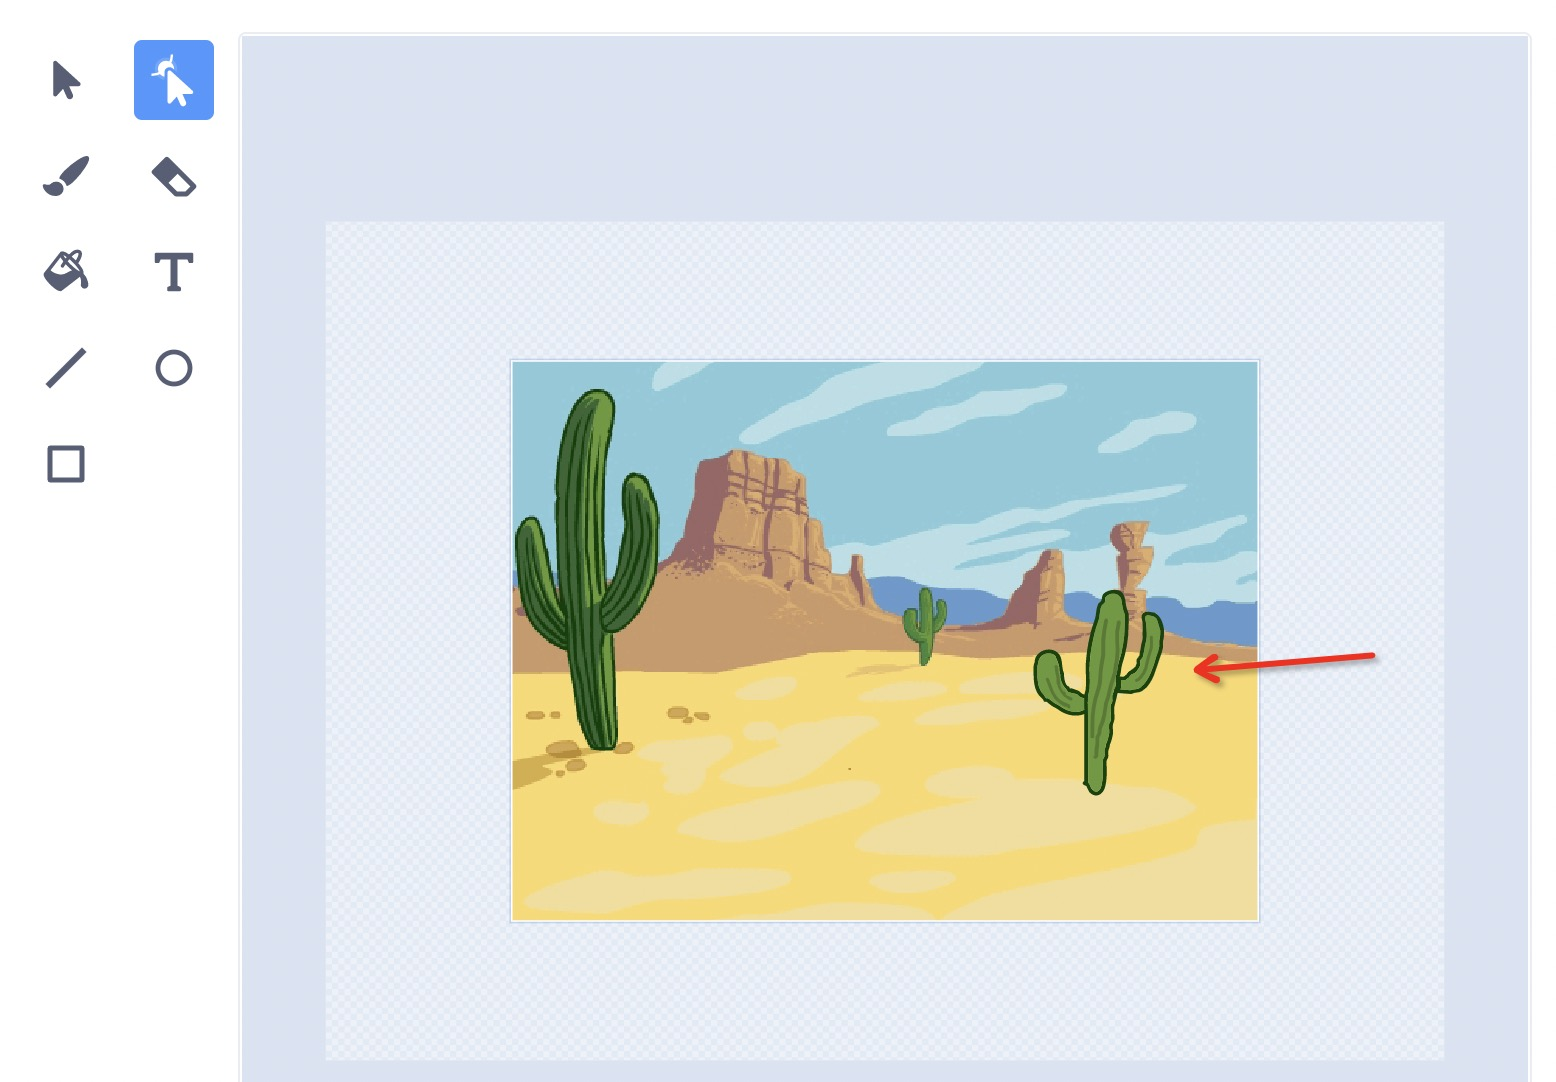
\includegraphics[width=\textwidth]{4.jpg}
                \caption*{第4题}
            \end{minipage}
            \begin{minipage}[t]{.24\textwidth}
                \centering
                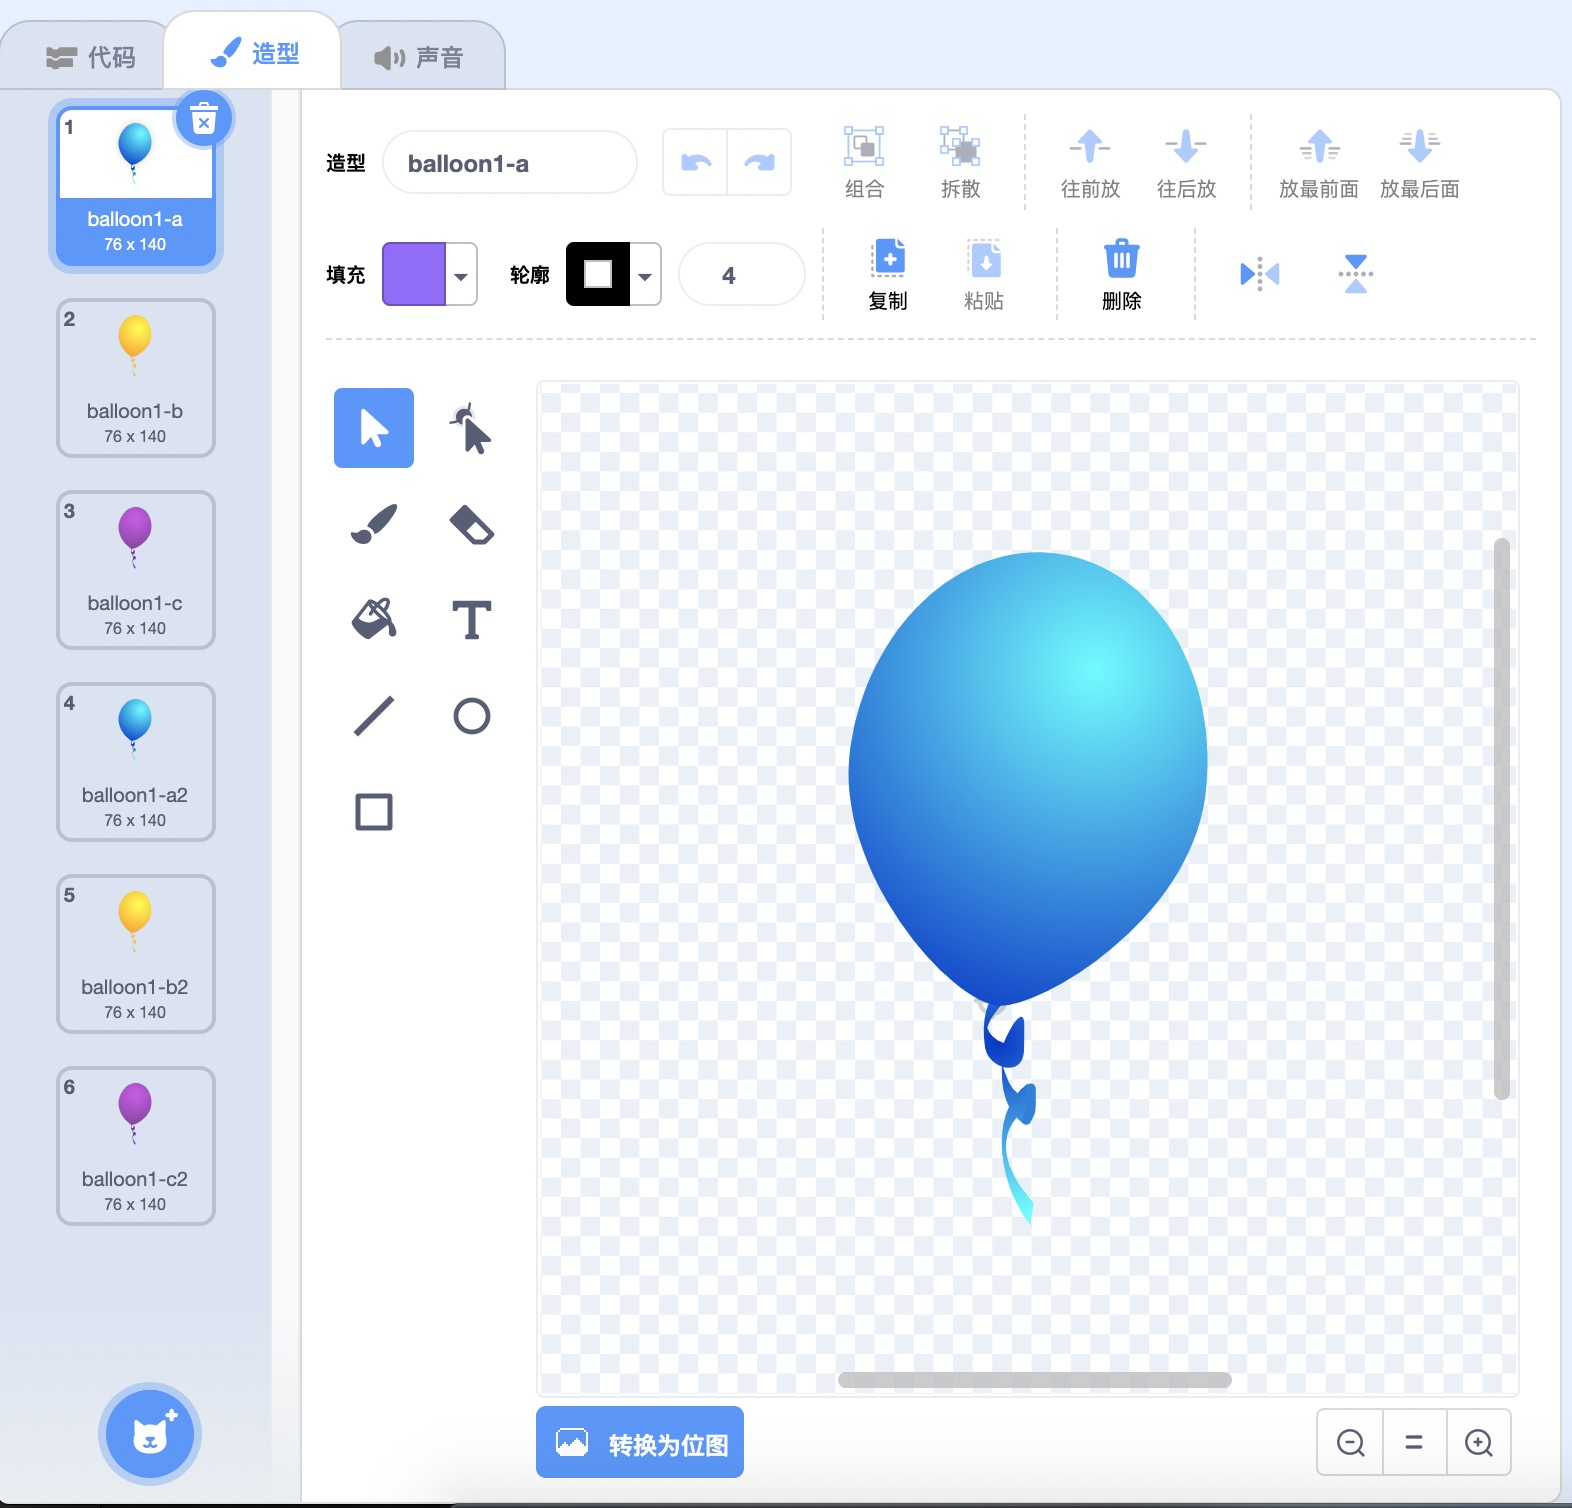
\includegraphics[width=\textwidth]{5.jpg}
                \caption*{第5题}
            \end{minipage}
        \end{figure}

        % 4
        \item 如上图,笑笑在沙漠中画了一个仙人掌。在画仙人掌的过程中,她有可能使用了哪个工具?(\qquad)
        \begin{tasks}(4)
            \task 
\includegraphics[width=.05\textwidth]{4a.jpg}
            \task 
\includegraphics[width=.05\textwidth]{4b.jpg}
            \task 
\includegraphics[width=.05\textwidth]{4c.jpg}
            \task 
\includegraphics[width=.05\textwidth]{4d.jpg}
        \end{tasks}

        % 5
        \item 如上图所示,角色一共有几个造型?(\qquad)
        \begin{tasks}(4)
            \task 3
            \task 4
            \task 5
            \task 6
        \end{tasks}

        % 6
        \item 舞台区如下图所示,将角色切换为哪个造型有可能出现运动员击中棒球的效果?(\qquad)
        
        \begin{minipage}{.25\textwidth}
            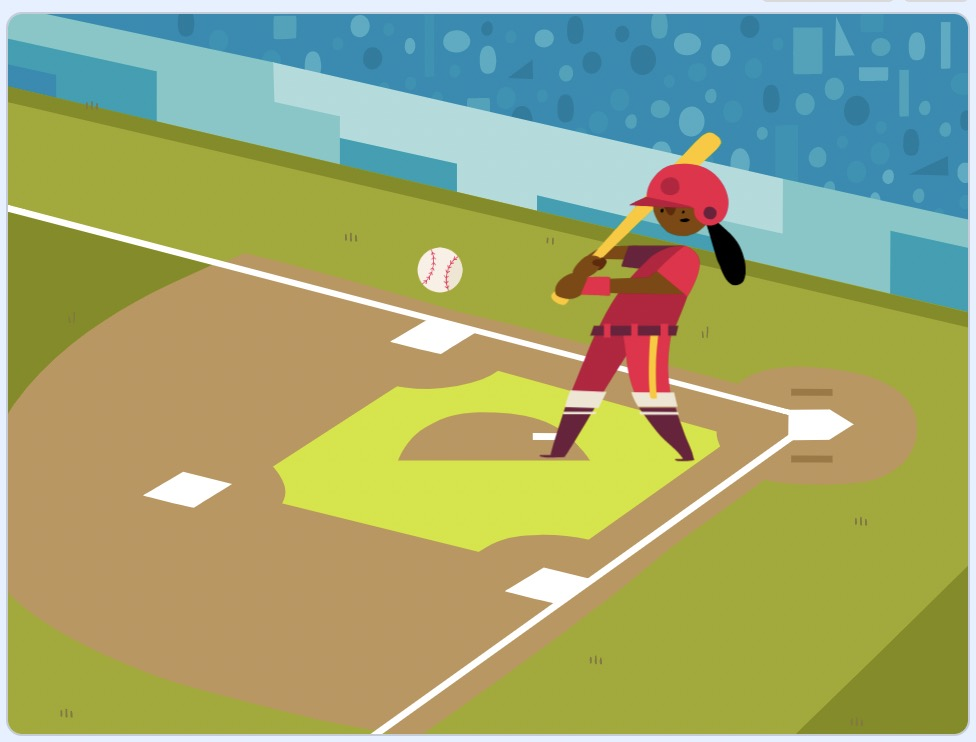
\includegraphics[width=0.6\textwidth]{6.jpg}
        \end{minipage}
        \begin{minipage}{.68\textwidth}
            \begin{tasks}(4)
                \task 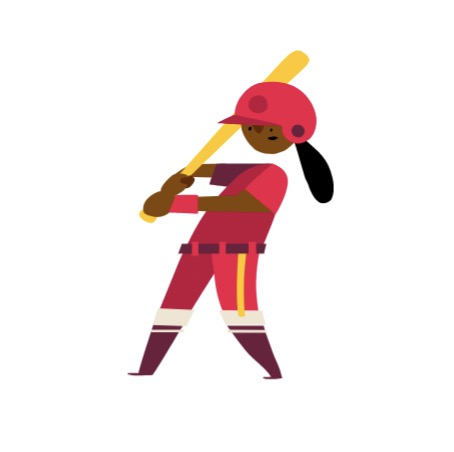
\includegraphics[width=.12\textwidth]{6a.jpg}
                \task 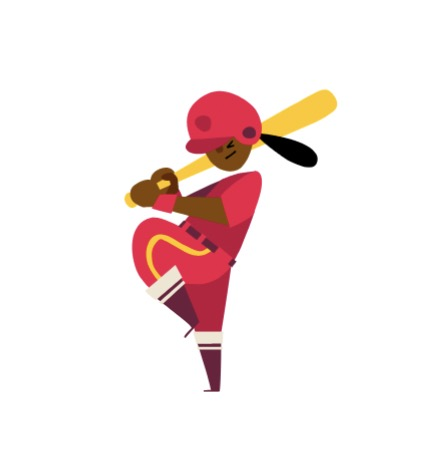
\includegraphics[width=.12\textwidth]{6b.jpg}
                \task 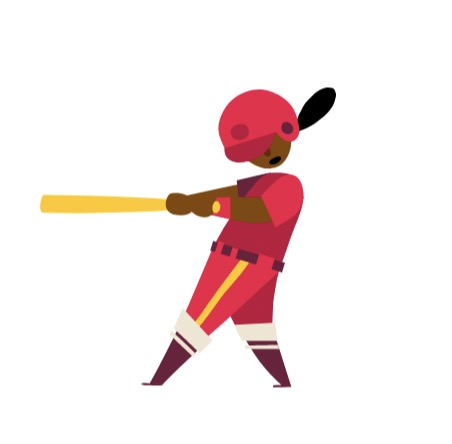
\includegraphics[width=.12\textwidth]{6c.jpg}
                \task 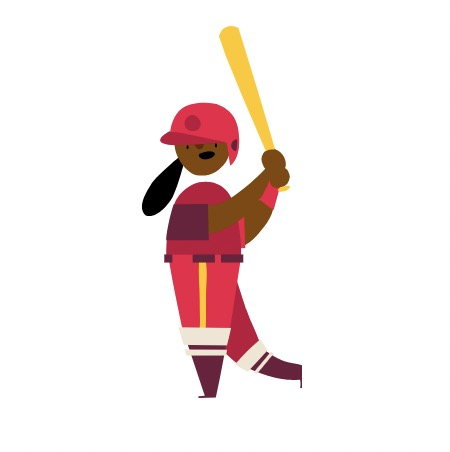
\includegraphics[width=.12\textwidth]{6d.jpg}
            \end{tasks}
        \end{minipage}
        

    % %     \newpage
        % 7
        \item 木木将自己旅游的照片上传到背景中,以下哪个积木不能实现照片切换?(\qquad)
        \begin{tasks}(4)
            \task 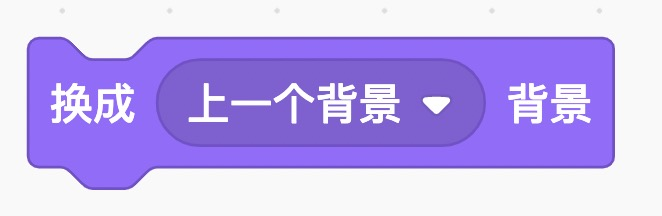
\includegraphics[width=.15\textwidth]{7a.jpg}
            \task 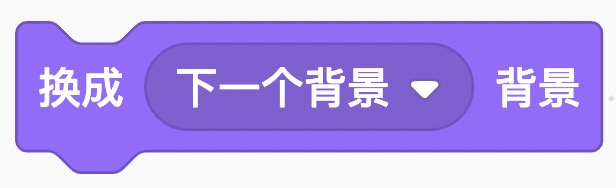
\includegraphics[width=.15\textwidth]{7b.jpg}
            \task 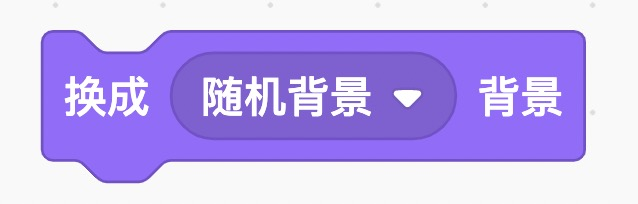
\includegraphics[width=.15\textwidth]{7c.jpg}
            \task 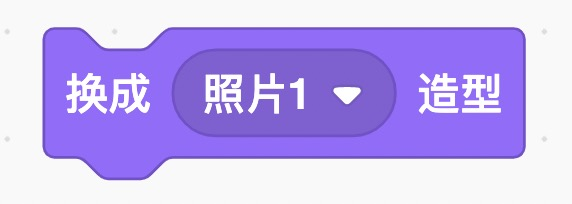
\includegraphics[width=.15\textwidth]{7d.jpg}
        \end{tasks}
           
        \newpage
        % 8
        \item 如下图,点击绿旗,下列描述正确的是?(\qquad)
        \begin{tasks}(2)
            \task 小女孩先向右移动了一段距离,然后开始跳舞
            \task 小女孩先跳舞,然后向右移动了一段距离
            \task 小女孩先向左移动了一段距离,然后跳舞
            \task 小女孩先跳舞,然后向左移动了一段距离
        \end{tasks}

        % 9
        \item 白马共6个造型,分别是白马奔跑时的拆解动作。执行下列哪个程序,可以让白马看起来跑得更快一些?(\qquad)
        \begin{tasks}(4)
            \task 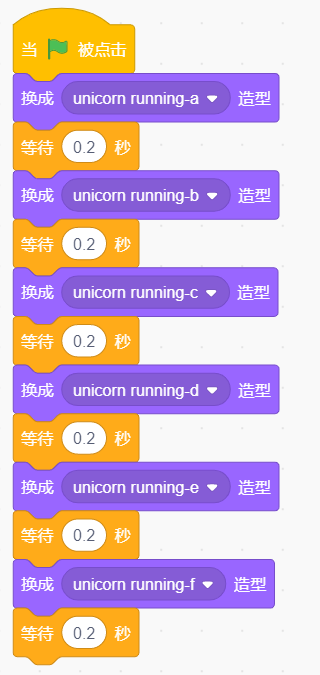
\includegraphics[width=.15\textwidth]{9a.png}
            \task 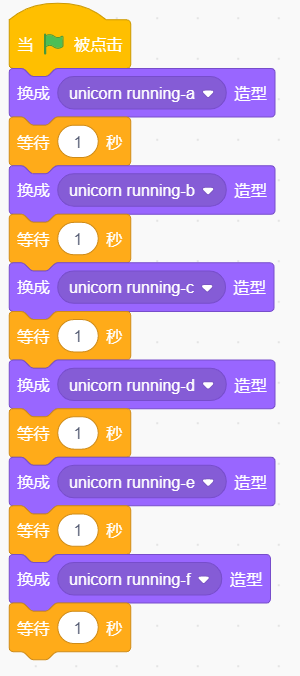
\includegraphics[width=.14\textwidth]{9b.png}
            \task 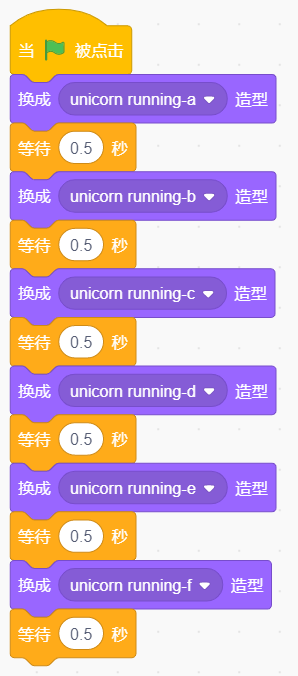
\includegraphics[width=.14\textwidth]{9c.png}
            \task 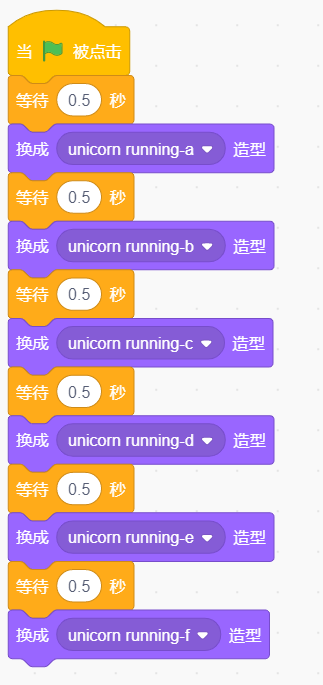
\includegraphics[width=.15\textwidth]{9d.png}
        \end{tasks}

        \begin{figure}[htbp]
            \begin{minipage}[t]{.48\textwidth}
                \centering
                \begin{minipage}{.4\textwidth}
                    \centering
                    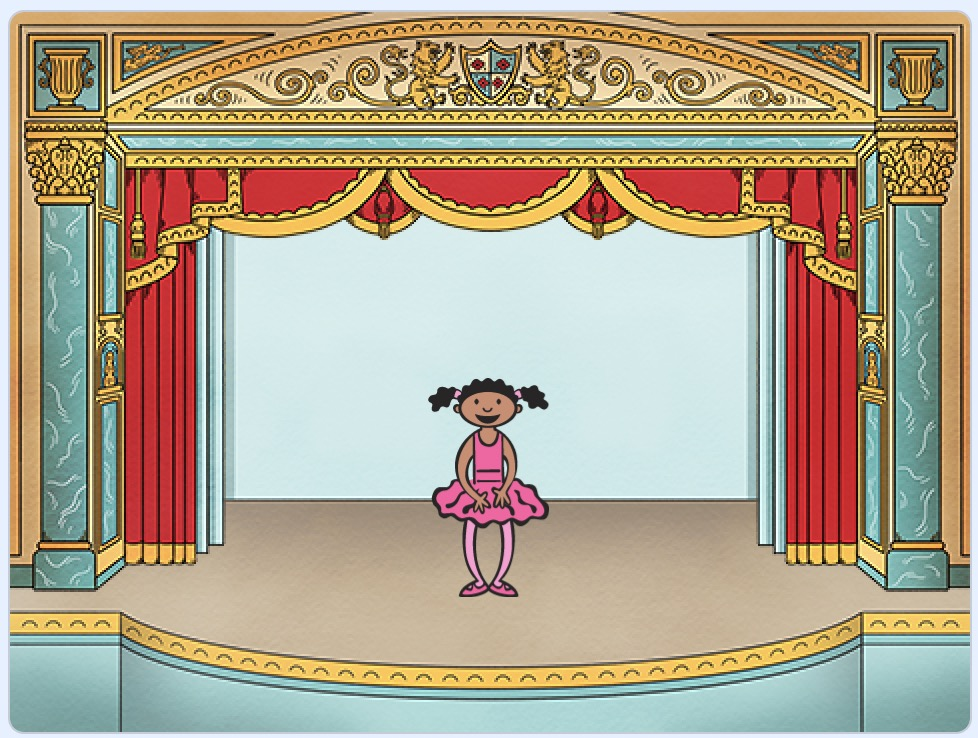
\includegraphics[width=\textwidth]{8.jpg}
                \end{minipage}
                \begin{minipage}{.28\textwidth}
                    \centering
                    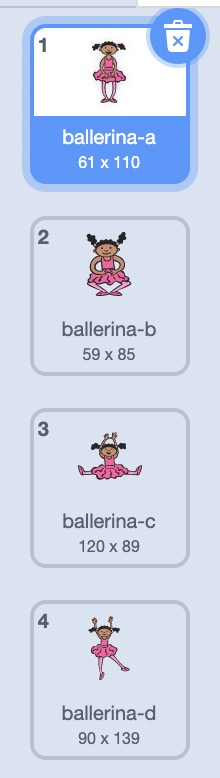
\includegraphics[width=.6\textwidth]{8-1.jpg}
                \end{minipage}
                \begin{minipage}{.28\textwidth}
                    \centering
                    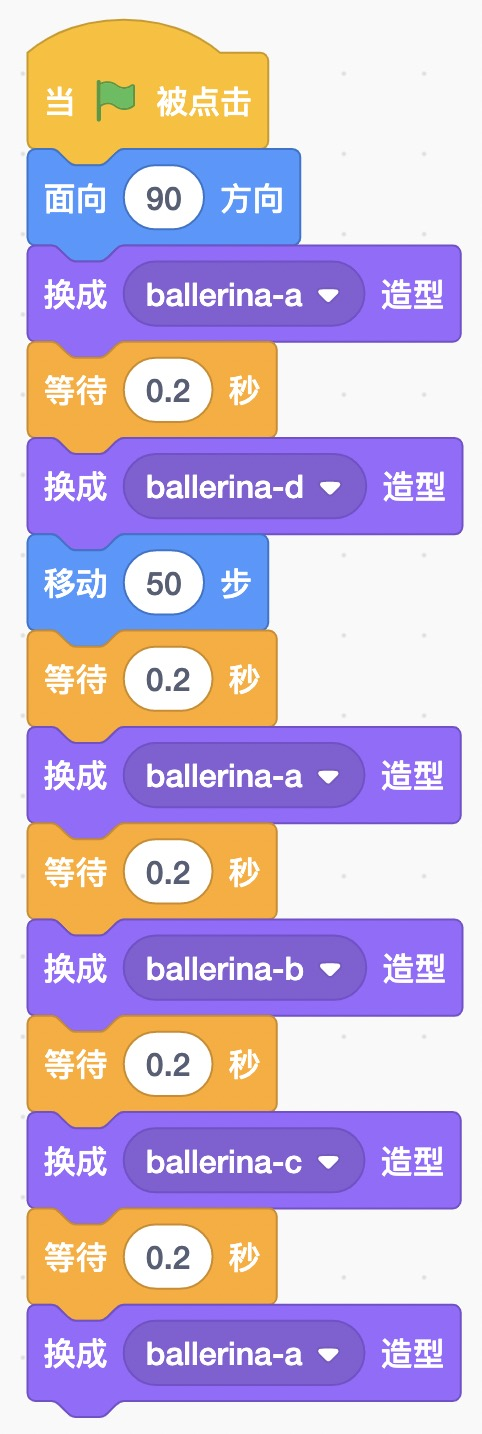
\includegraphics[width=.7\textwidth]{8-2.jpg}
                \end{minipage}
                \caption*{第8题}
            \end{minipage}
            \begin{minipage}[t]{.48\textwidth}
                \centering
                \begin{minipage}{.3\textwidth}
                    \centering
                    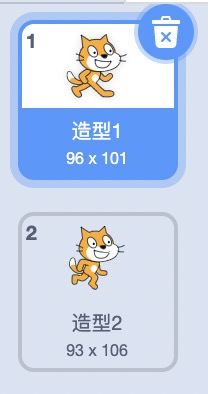
\includegraphics[width=\textwidth]{10-1.png}
                \end{minipage}
                \begin{minipage}{.4\textwidth}
                    \centering
                    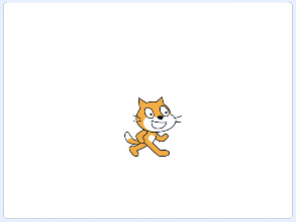
\includegraphics[width=\textwidth]{10-2.png}
                \end{minipage}
                \begin{minipage}{.25\textwidth}
                    \centering
                    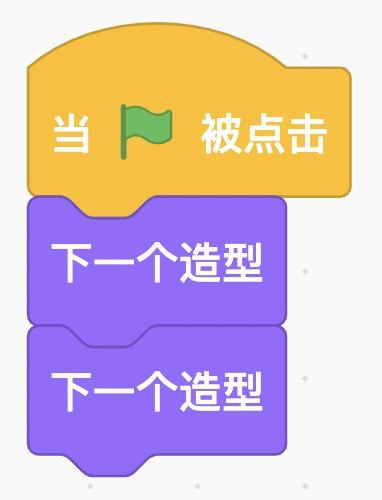
\includegraphics[width=\textwidth]{10-3.png}
                \end{minipage}
                \caption*{第10题}
            \end{minipage}
        \end{figure}

        % 10
        \item 如上图,点击绿旗后,下列描述不正确的是?(\qquad)
        \begin{tasks}
            \task 程序运行后,看不到小猫有任何变化
            \task 程序运行结束后,小猫还是原来的造型
            \task 程序运行过程中,小猫切换了2次造型,速度太快,看不出造型变化
            \task 程序运行后,小猫变成了“造型2”
        \end{tasks}

        % 11
        \item 汽车的初始位置如下图所示,点击一次绿旗,下列哪个选项可以让汽车从舞台左侧移动到右侧?(\qquad)
        
        \begin{minipage}{.2\textwidth}
            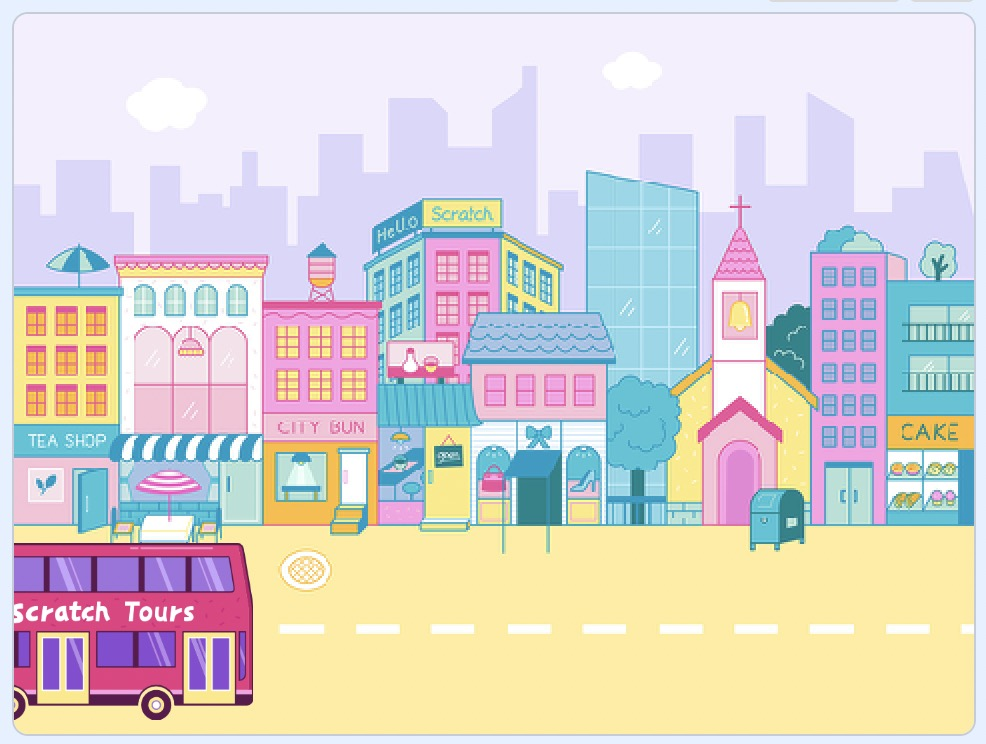
\includegraphics[width=\textwidth]{11.jpg}
        \end{minipage}
        \begin{minipage}{.73\textwidth}
            \begin{tasks}(4)
                \task 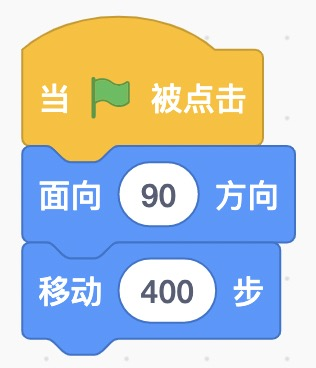
\includegraphics[width=.11\textwidth]{11a.jpg}
                \task 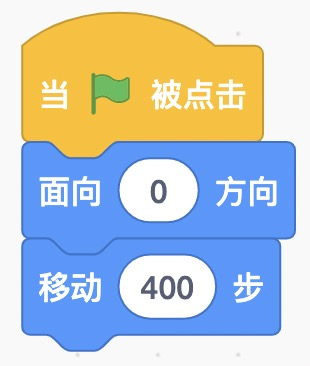
\includegraphics[width=.11\textwidth]{11b.jpg}
                \task 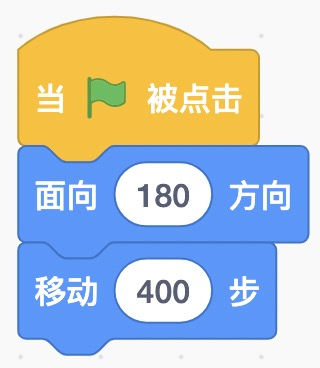
\includegraphics[width=.11\textwidth]{11c.jpg}
                \task 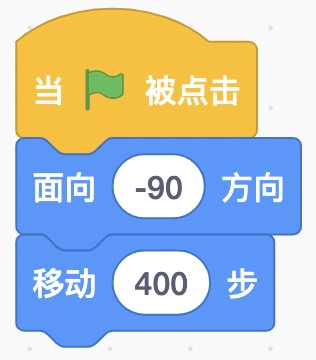
\includegraphics[width=.11\textwidth]{11d.jpg}
            \end{tasks}
        \end{minipage}
        
        % 12
        \item 积木块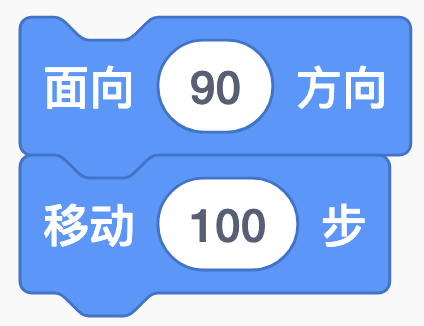
\includegraphics[width=.08\textwidth]{12.png}属于哪个模块?(\qquad)
        \begin{tasks}(4)
            \task 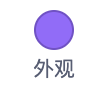
\includegraphics[width=.06\textwidth]{12a.png}
            \task 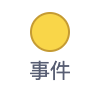
\includegraphics[width=.06\textwidth]{12b.png}
            \task 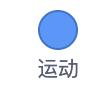
\includegraphics[width=.06\textwidth]{12c.png}
            \task 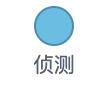
\includegraphics[width=.06\textwidth]{12d.png}
        \end{tasks}

        \newpage
        % 13
        \item 如下图,蝴蝶从现在的位置飞到右下角的花上,在起飞前,需要调整的方向是?(\qquad)
        \begin{tasks}(4)
            \task 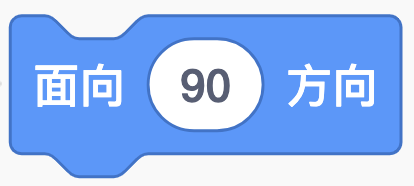
\includegraphics[width=.1\textwidth]{13a.png}
            \task 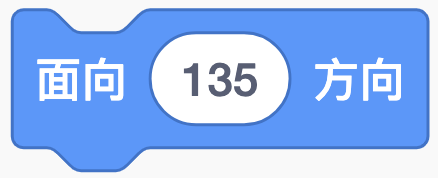
\includegraphics[width=.1\textwidth]{13b.png}
            \task 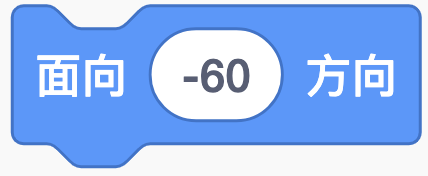
\includegraphics[width=.1\textwidth]{13c.png}
            \task 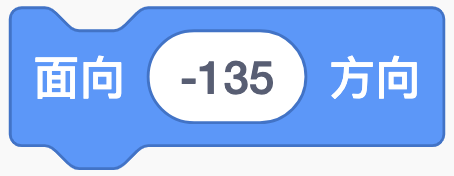
\includegraphics[width=.1\textwidth]{13d.png}
        \end{tasks}

        % 14
        \item 如下图,点击绿旗后,星星的方向和大小分别是多少?(\qquad)
        \begin{tasks}(2)
            \task 面向90方向,大小为60
            \task 面向-150方向,大小为160
            \task 面向60方向,大小为60
            \task 面向180方向,大小为160
        \end{tasks}

        \begin{figure}[htbp]
            \centering
            \begin{minipage}[t]{.25\textwidth}
                \centering
                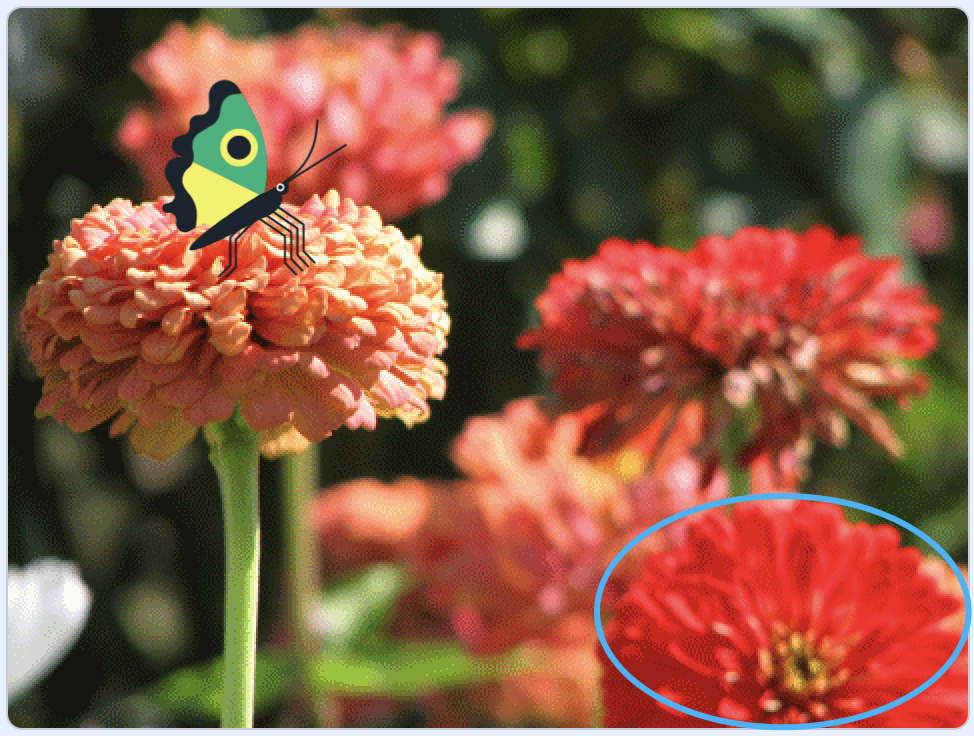
\includegraphics[width=\textwidth]{13.png}
                \caption*{第13题}
            \end{minipage}
            \begin{minipage}[t]{.35\textwidth}
                \centering
                \begin{minipage}[t]{.7\textwidth}
                    \centering
                    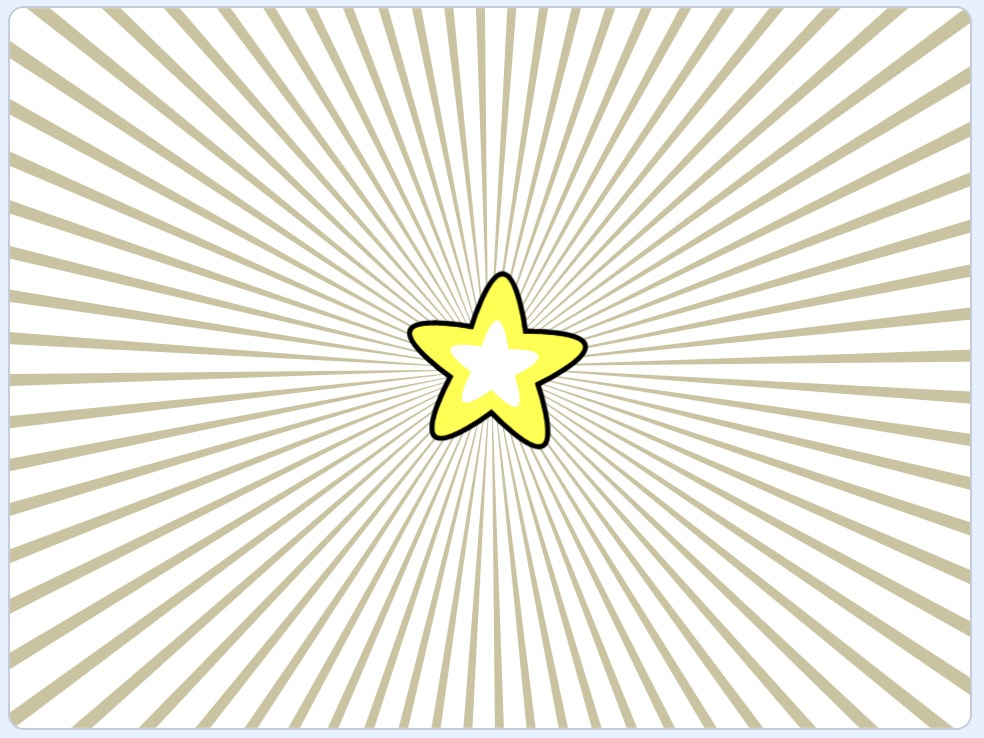
\includegraphics[width=\textwidth]{14.jpg}
                \end{minipage}
                \begin{minipage}[t]{.25\textwidth}
                    \centering
                    \includegraphics[width=\textwidth]{14-1.jpg}
                \end{minipage}
                \caption*{第14题}
            \end{minipage}
            \begin{minipage}[t]{.25\textwidth}
                \centering
                \includegraphics[width=\textwidth]{16.jpg}
                \caption*{第16题}
            \end{minipage}
            \begin{minipage}[t]{.11\textwidth}
                \centering
                \includegraphics[width=\textwidth]{17.png}
                \caption*{第17题}
            \end{minipage}
        \end{figure}
    
        % 15
        \item 以下哪个选项不是角色的旋转方式?(\qquad)
        \begin{tasks}(4)
            \task 不可旋转
            \task 左右翻转
            \task 任意旋转
            \task 前后翻转
        \end{tasks}

        % 16
        \item 在上图区域内不能完成的操作是?(\qquad)
        \begin{tasks}(4)
            \task 上传一个角色
            \task 修改角色名称
            \task 修改造型名称
            \task 复制一个角色
        \end{tasks}

        % 17
        \item 角色的初始方向为90,位置在舞台中心,执行一次上图程序后,角色的最终位置距离初始位置多少步?(\qquad)
        \begin{tasks}(4)
            \task 16
            \task 18
            \task 10
            \task 19
        \end{tasks}

        % 18
        \item 下列哪个按钮能让声音大一些?(\qquad)
        \begin{tasks}(4)
            \task \includegraphics[width=.05\textwidth]{18a.jpg}
            \task \includegraphics[width=.05\textwidth]{18b.jpg}
            \task \includegraphics[width=.05\textwidth]{18c.jpg}
            \task \includegraphics[width=.05\textwidth]{18d.jpg}
        \end{tasks}

        % 19
        \item 角色的程序如下图所示,声音“Cymbal”的时长为1秒,声音“Techno”的时长为7秒。点击绿旗,下列选项描述正确的是?(\qquad)
        
        \begin{minipage}{.37\textwidth}
            \includegraphics[width=\textwidth]{19.jpg}
        \end{minipage}
        \begin{minipage}{.57\textwidth}
            \begin{tasks}
                \task 第2段“Techno”不会播放
                \task 第2段“Techno”播放时,没有其他声音在同时播放
                \task 程序运行过程中,有2秒的时间是没有任何声音播放的
                \task 这个程序运行14秒后结束
            \end{tasks}
        \end{minipage}
        

        % 20
        \item 下列哪个积木能改变声音的音量?(\qquad)
        \begin{tasks}(4)
            \task \includegraphics[width=.18\textwidth]{20a.jpg}
            \task \includegraphics[width=.18\textwidth]{20b.jpg}
            \task \includegraphics[width=.18\textwidth]{20c.jpg}
            \task \includegraphics[width=.18\textwidth]{20d.jpg}
        \end{tasks}

        \newpage
        % 21
        \item 下列哪个选项的积木可以停止正在播放中的声音?(\qquad)
        \begin{tasks}(2)
            \task \includegraphics[width=.13\textwidth]{21a1.png}和\includegraphics[width=.09\textwidth]{21a2.png}都可以停止声音
            \task \includegraphics[width=.13\textwidth]{21b1.png}和\includegraphics[width=.07\textwidth]{21b2.png}都可以停止声音
            \task \includegraphics[width=.13\textwidth]{21c.png}
            \task \includegraphics[width=.1\textwidth]{21d.png}
        \end{tasks}

        % 22
        \item 如图\includegraphics[width=.15\textwidth]{22.jpg}所示积木的结果是多少?(\qquad)
        \begin{tasks}(4)
            \task 4
            \task 3
            \task 7
            \task 6
        \end{tasks}

        % 23
        \item 一共有9个小朋友分一个生日蛋糕,最少切几刀可以保证每个小朋友至少能分到一块蛋糕?(\qquad)
        \begin{tasks}(4)
            \task 3
            \task 4
            \task 5
            \task 6
        \end{tasks}

        % 24
        \item 小青、小峰、小林和小方四个人比身高,小青说“我比小峰高”,小林说“小方比小峰矮”,小方说“小林比我矮”。将四个人按照身高从高到矮进行排序。正确的顺序是?(\qquad)
        \begin{tasks}(2)
            \task 小青、小峰、小方、小林
            \task 小青、小方、小峰、小林
            \task 小峰、小青、小林、小方
            \task 小峰、小方、小青、小林
        \end{tasks}
        
        % 25
        \item 如下图所示,天平左边有5克、4克和3克的砝码,右边有7克、6克和5克的砝码,怎样调整砝码可以让天平保持平衡?(\qquad)
        \begin{tasks}(2)
            \task 将右边的7克砝码拿掉
            \task 在左边添加一个5克的砝码
            \task 将左边的3克砝码和右边的6克砝码对调
            \task 将左边的3克砝码和右边的7克砝码对调
        \end{tasks}

        \begin{figure}[htbp]
            \centering
            \begin{minipage}[t]{.23\textwidth}
                \centering
                \includegraphics[width=\textwidth]{25.png}
                \caption*{第25题}
            \end{minipage}
            \begin{minipage}[t]{.33\textwidth}
                \centering
                \includegraphics[width=\textwidth]{29.jpg}
                \caption*{第29题}
            \end{minipage}
            \begin{minipage}[t]{.28\textwidth}
                \centering
                \includegraphics[width=\textwidth]{33.jpg}
                \caption*{第33题}
            \end{minipage}
        \end{figure}
    \end{enumerate}

    {\noindent\heiti 第二部分、判断题(共 10 题,每题 2 分,共20分.)}
    \begin{enumerate}
        \setcounter{enumi}{25}
        % 26
        \item 在创作编程作品时,可以根据作品内容上传或绘制合适的背景、角色和造型.(\qquad)

        %27
        \item 在同一个编程作品中不能有同名的角色,但在同一个角色下,可以有同名的造型.(\qquad)
        
        %28
        \item 切换角色造型或舞台背景,只能在代码区中通过编程实现.(\qquad)
  
        %29
        \item 如上图,在角色库中添加的角色是不能修改造型的.(\qquad)
        
        %30
        \item 角色复制后,角色名称不同但造型名称相同.(\qquad)
        
        %31
        \item 导出角色的造型时,可以将角色中编好的程序一起导出来.(\qquad)
        
        %32
        \item 角色旋转720°后,面向的方向与初始方向一致.(\qquad)
        
        %33
        \item 执行如上图程序时,可以同时听到两段声音.(\qquad)
        
        \newpage
        %34
        \item 创作作品时,可以从声音库中选择一段声音,也自己录制一段声音,但不能上传音频文件.(\qquad)
        
        %35
        \item 一壶水可以装满8个杯子,一壶水可以装满4个碗。那么一杯水可以装满2个碗.(\qquad)
    \end{enumerate}

    {\noindent\heiti 第三部分、编程题(共 2 题,共30分.)}
    \begin{enumerate}
        \setcounter{enumi}{35}
        
        % 36
        \item 放学:
        
        1. 准备工作
        \begin{tasks}[label = (\arabic*)]
            \task 添加背景:School;
            \task 删除默认的小猫角色,添加角色:City Bus、Kai;
            \task 为角色City Bus添加声音:Car Horn;
        \end{tasks}
        2. 功能实现
        \begin{tasks}[label = (\arabic*)]
            \task 点击绿旗,City Bus出现在舞台左下角,Kai出现在学校门口;
            \task City Bus向前移动一段距离,连续播放两次声音Car Horn;
            \task 听到声音后,Kai调整方向,走到车门的位置后消失; 
            \task City Bus继续向前行驶直到舞台右侧。
        \end{tasks}
        \begin{figure}[htbp]
            \centering
            \begin{minipage}{.2\textwidth}
                \centering
                \includegraphics[width=\textwidth]{361.jpg}
            \end{minipage}
            \begin{minipage}{.2\textwidth}
                \centering
                \includegraphics[width=\textwidth]{36-2.jpg}
            \end{minipage}
            \begin{minipage}{.2\textwidth}
                \centering
                \includegraphics[width=\textwidth]{36-3.jpg}
            \end{minipage}
            \begin{minipage}{.2\textwidth}
                \centering
                \includegraphics[width=\textwidth]{36-5.jpg}
            \end{minipage}
        \end{figure}

        %37
        \item 下雨:
        
        1. 准备工作
        \begin{tasks}[label = (\arabic*)]
            \task 添加背景:Room 2、Witch House;
            \task 删除默认的小猫角色,添加角色:Abby、Dani。
        \end{tasks}
        2. 功能实现
        \begin{tasks}[label = (\arabic*)]
            \task 点击绿旗,舞台背景切换为Room 2,Abby出现在舞台左侧,面向右,Dani出现在舞台右侧,面向左;
            \task Abby说“外面在下雨吗?”2秒,Abby说完后,Dani说“我去看一下”2秒,Dani说完后,转身走到舞台右侧边缘的位置;
            \task 舞台背景切换为Witch House,Abby角色消失,Dani出现在舞台左下角;
            \task Dani走到到窗户旁边,说“没有下雨”2秒。
        \end{tasks}

        \begin{figure}[htb]
            \centering
            \begin{minipage}[t]{.2\textwidth}
                \centering
                \includegraphics[width=\textwidth]{37-1.jpg}
            \end{minipage}
            \begin{minipage}[t]{.2\textwidth}
                \centering
                \includegraphics[width=\textwidth]{37-2.jpg}
            \end{minipage}
            \begin{minipage}[t]{.2\textwidth}
                \centering
                \includegraphics[width=\textwidth]{37-3.jpg}
            \end{minipage}
            \begin{minipage}[t]{.2\textwidth}
                \centering
                \includegraphics[width=\textwidth]{37-4.jpg}
            \end{minipage}
        \end{figure}
    \end{enumerate}
\end{document}